\documentclass[11pt]{article}
\usepackage[margin=1in]{geometry}
\usepackage{volfit_preamble}
\graphicspath{{figures/}}

\title{\textbf{Spot--Vol Dynamics: SSR and Smile Transport}\\[2pt]
\large Moving the smile when spot moves, without recalibration\\[2pt]
\normalsize Vol-Fitter Technical Notes, No.~12}
\author{Vol-Fitter}
\date{\today}

\begin{document}
\maketitle
% Auto-generated by gen_ssr.py — do not edit.
\newcommand{\ssrskew}{-0.353}
\newcommand{\ssrmove}{-5}


\begin{abstract}
When the underlying moves, the implied-volatility smile moves with it, and a desk
must know \emph{how} --- to risk-manage, to scenario, and to refresh a surface
between calibrations. This note documents the Vol-Fitter's spot--vol dynamics. The
organizing quantity is the skew-stickiness ratio
$\mathrm{SSR}=(\dd\sigma_{\text{atm}}/\dd\ln F)/\text{skew}$, the fraction of the
skew realized as an ATM-vol change per unit log-spot move. Three canonical regimes
fix it: sticky-moneyness ($\mathrm{SSR}=0$, the smile rides with the forward),
sticky-strike ($\mathrm{SSR}=1$, vol fixed at each strike), and sticky-local-vol
($\mathrm{SSR}\approx2$ for short-dated skews). We give the analytic transport that
realizes any SSR in one line, derive its ATM response, and then the \emph{exact}
sticky-local-vol transport (a Hagan-style log-moneyness displacement) and the
local-vol-grid relabeling that implements it by simply re-indexing the surface's
strike nodes. Every relabeling path is recalibration-free --- a spot move refreshes
the surface by arithmetic, not by re-solving; the one exception is the exact
sticky-local-vol-grid \emph{reprice}, which pays for its exactness with a single
Dupire PDE solve and is chosen explicitly when exactness is wanted over speed. A
worked example transports an equity smile under a $\ssrmove\%$ move in the three
regimes.
\end{abstract}

\tableofcontents
\newpage

%======================================================================
\section{The question}
\label{sec:question}

A calibrated surface is a snapshot at one spot. The next tick moves spot, and the
desk needs the new smile \emph{now} --- faster than a recalibration, and consistent
with a chosen dynamics assumption. The assumptions differ in how much the ATM vol
follows the skew as spot moves, and the summary statistic is the
\emph{skew-stickiness ratio}
\begin{equation}
\mathrm{SSR}=\frac{\dd\sigma_{\text{atm}}/\dd\ln F}{s_0},
\qquad s_0=\left.\frac{\partial\sigma}{\partial k}\right|_{k=0}\ (\text{the ATM skew}).
\label{eq:ssr}
\end{equation}

\begin{heuristic}
Read SSR as ``how much of the skew is real''. The skew $s_0$ says that lower
strikes have higher vol. When spot drops, does the ATM vol rise to where the old
lower-strike vol was (SSR$=1$, sticky-strike), not move at all in moneyness terms
(SSR$=0$, sticky-moneyness), or \emph{overshoot} (SSR$\approx2$, sticky-local-vol,
the empirically common short-dated regime)? SSR interpolates these, and the
transport below realizes any value of it.
\end{heuristic}

%======================================================================
\section{Conventions, fixed once}
\label{sec:conventions}

Every sign error in smile transport comes from mixing two coordinate systems,
so we fix the conventions once, and every formula in this note (and in the
code, sign-for-sign) follows them:

\begin{assumption}[Sign conventions]
\label{ass:signs}
(i) The move is $h=\delta=\ln(F_{\text{new}}/F_{\text{old}})$: positive when
the forward rises. (ii) Log-moneyness $k=\log(K/F)$ is always measured
against the \emph{prevailing} forward --- so the same absolute strike has
\emph{lower} moneyness after an up-move: $k_{\text{new}}=k_{\text{old}}-h$.
(iii) A transported \emph{curve} is a function of new moneyness; a
transported \emph{quote} (a fixed strike) is a point whose moneyness label
changes.
\end{assumption}

Convention (ii) is where the classic off-by-sign lives, because it makes
curves and quotes move in \emph{opposite} directions in $k$:

\begin{caution}
Under sticky-strike, the vol at each fixed strike is unchanged. To express
the \emph{new curve} at new moneyness $k$, ask which old strike now sits
there: the strike whose old moneyness was $k+\delta$. Hence the curve
transport reads \emph{forward}, $\sigma_{\text{new}}(k)=
\sigma_{\text{old}}(k+\delta)$ --- a \emph{plus}. But re-labelling an
existing fixed-strike quote goes the other way: its new moneyness is
$k-h$ --- a \emph{minus}. Both signs are correct, both are in production
(the smile transport uses $k+\delta$; the local-vol view re-indexes stored
quotes by $k-h$), and swapping either one flips the skew response. The
sign-locking tests below are the fence.
\end{caution}

%======================================================================
\section{The analytic transport}
\label{sec:transport}

Let $h=\delta=\ln(F_{\text{new}}/F_{\text{old}})$ be the log-forward move and
$\sigma_{\text{old}}(k)$ the pre-move smile in log-moneyness. The Vol-Fitter
transports the smile to new-forward moneyness $k$ by
\begin{equation}
\boxed{\;\sigma_{\text{new}}(k)=\sigma_{\text{old}}(k+\delta)+(\mathrm{SSR}-1)\,s_0\,\delta.\;}
\label{eq:shift}
\end{equation}
The first term is a \emph{sticky-strike re-indexing} (a strike that was at
moneyness $k+\delta$ before the move is at moneyness $k$ after it); the second is a
uniform \emph{level adjustment} that dials in the desired ATM response while
preserving the smile shape. The transport \eqref{eq:shift} is literally one line
(matches production to $10^{-13}$):

\begin{lstlisting}[caption={The SSR smile transport \eqref{eq:shift} for any
regime (distilled from \texttt{dynamics/ssr.py}; production's last argument
is a \texttt{regime} accepting a named regime or a numeric SSR).},
label={lst:ssr}]
def shifted_smile(k, vol_curve, atm_skew, spot_return, ssr):
    d = np.log1p(spot_return)                        # delta = log(F_new/F_old)
    return vol_curve(k + d) + (ssr - 1.0)*atm_skew*d # curve reindex + level adj
\end{lstlisting}

\begin{proposition}[ATM response]
\label{prop:atm}
Under \eqref{eq:shift}, to first order in $\delta$ the ATM vol moves by
$\Delta\sigma_{\text{atm}}=\mathrm{SSR}\cdot s_0\cdot\delta$, consistent with the
SSR definition \eqref{eq:ssr}.
\end{proposition}

\begin{proof}
At $k=0$, $\sigma_{\text{new}}(0)=\sigma_{\text{old}}(\delta)+(\mathrm{SSR}-1)s_0\delta
=\sigma_{\text{old}}(0)+s_0\delta+(\mathrm{SSR}-1)s_0\delta+O(\delta^2)
=\sigma_{\text{old}}(0)+\mathrm{SSR}\,s_0\delta+O(\delta^2)$.
\end{proof}

So $\mathrm{SSR}=0$ leaves the smile a pure function of moneyness (sticky-moneyness:
$\Delta\sigma_{\text{atm}}=0$), $\mathrm{SSR}=1$ cancels the level term and freezes
vol at each strike (sticky-strike), and $\mathrm{SSR}=2$ doubles the skew's
contribution. \Cref{fig:transport} transports an equity smile (ATM skew
$s_0=\ssrskew$) under a $\ssrmove\%$ move in all three regimes;
\cref{fig:response} shows the linear ATM responses of slope $\mathrm{SSR}\,s_0$.

\begin{figure}[H]
\centering
\begin{minipage}{0.52\textwidth}\centering
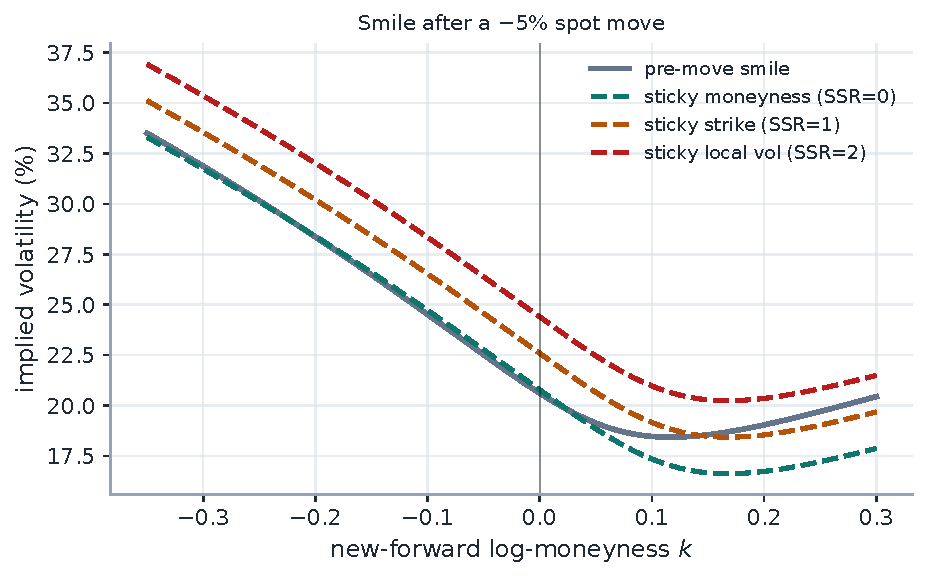
\includegraphics[width=\textwidth]{fig_ssr_transport.pdf}\\[1pt]
{\footnotesize (a) transported smiles}
\end{minipage}\hfill
\begin{minipage}{0.45\textwidth}\centering
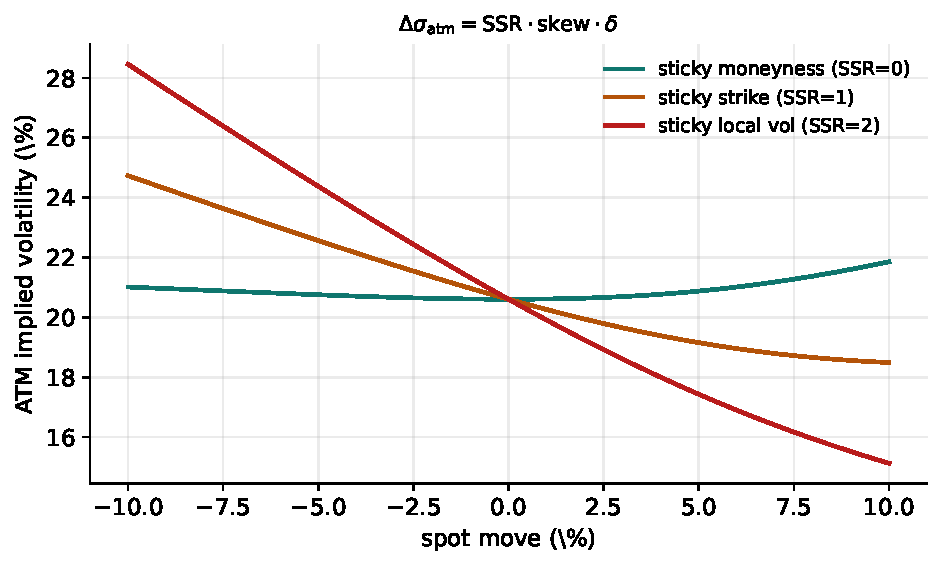
\includegraphics[width=\textwidth]{fig_ssr_response.pdf}\\[1pt]
{\footnotesize (b) ATM response vs spot move}
\end{minipage}
\caption{Transporting an equity smile under a $\ssrmove\%$ spot move in the three
canonical regimes. The ATM response is linear with slope $\mathrm{SSR}\cdot s_0$.}
\label{fig:transport}
\end{figure}
\begin{figure}[H]\centering\phantomsection\label{fig:response}\end{figure}

%======================================================================
\section{Exact sticky-local-vol}
\label{sec:exactlv}

The shift \eqref{eq:shift} is a first-order, shape-preserving approximation. For
the \emph{sticky-local-vol} regime there is an \emph{exact} transport, because
holding the local-volatility function fixed in absolute strike determines the new
implied surface completely. In total-variance form, the horizontal-SSR transport is
\begin{equation}
\widetilde w_1^{R}(T,k)=w_0\big(T,\;k+R\,h_T\big),
\end{equation}
and the exact sticky-local-vol transport replaces the linear displacement by the
Hagan log-moneyness map
\begin{equation}
w_1^{\text{LV}}(T,k)=w_0\big(T,\;\ell_T(k,h)\big),
\qquad \ell_T(k,h)=\log\!\big(e^{h}(e^{k}+1)-1\big),
\label{eq:hagan}
\end{equation}
which is the exact relabeling of moneyness when the local-vol surface is held fixed
in absolute strike and the forward moves by $h$. An optional ATM re-anchor
$\sigma_{\text{atm}}\to\sigma_0+R\,\kappa_T h_T$ makes the linear SSR response exact
even for large moves.

Expanding the Hagan map for a small move exposes where the famous ``$\approx2$''
comes from:
\begin{equation}
\ell_T(k,h)=k+\big(1+e^{-k}\big)\,h+O(h^2),
\qquad\text{so}\qquad
\ell_T(0,h)\approx 2h .
\label{eq:ellexpand}
\end{equation}
Holding the local-vol surface fixed makes the new smile read the old curve
\emph{two} units of log-moneyness per unit forward move at the money --- twice the
sticky-strike displacement of $\delta$ in \eqref{eq:shift} --- so the ATM vol picks
up $2\,s_0\,h$ to first order: the short-dated $\mathrm{SSR}\approx2$ of
\cref{sec:question} is not an empirical accident but the ATM slope of the exact
relabeling \eqref{eq:hagan}. Away from the money the displacement $(1+e^{-k})h$ is
strike-dependent --- larger on the put wing, smaller on the call wing --- which is
what the linear shift \eqref{eq:shift} deliberately flattens into a single level
adjustment. The expansion is test-locked (traceability table).

\subsection{The local-vol-grid relabeling}

When the dynamics are driven by the extracted local-vol \emph{grid} (Note~04), the
transport is even simpler: it is a \emph{relabeling of the grid's strike nodes}. A
grid node at absolute strike $K_i^0(t)$ moves to
\begin{equation}
K_i^{1,R}(t)=K_i^0(t)\,e^{(1-R/2)h_t},
\qquad\Longleftrightarrow\qquad
x_i^1=x_i^0-\tfrac{R}{2}\,h_t,
\label{eq:gridrelabel}
\end{equation}
in forward-normalized moneyness $x$. For $R=2$ (sticky-local-vol) the factor is
$e^{0}=1$: the grid is held fixed in absolute strike and re-priced through the
Dupire PDE, which is the \emph{exact} dynamics --- here SSR is an \emph{output} of
the reprice, not an input, and the value $2$ is only its short-maturity limit
\eqref{eq:ellexpand}. The exactness is not free: this reprice is the one path in
the note that is \emph{not} re-solve-free --- it costs a single Dupire PDE solve
(Note~04), whereas every relabeling path (\eqref{eq:shift}, \eqref{eq:hagan},
\eqref{eq:gridrelabel}) remains pure arithmetic. For
$R=0$ (sticky-moneyness) the grid scales with the forward; $R=1$ (sticky-strike)
sits halfway. This is why the local-vol regime is labeled both
\texttt{sticky\_local\_vol} (the analytic Hagan transport) and
\texttt{sticky\_local\_vol\_grid} (the exact PDE reprice).

In production the local-vol \emph{view} applies all three conventions of
\cref{ass:signs} at once, per read: each reconstructed smile is wrapped in
the curve transport (the $k+\delta$ rule), stored fixed-strike quotes are
re-indexed to $k-h$ (the quote rule), and the shared strike-node axis is
relabelled by $x\mapsto x\,e^{-(R/2)h}$ using the longest expiry's $h$ as the
representative move. The three signs are independently test-locked; the grid
rule in particular is pinned to the exact triple $(x,\ x-\tfrac12H,\ x-H)$
for the three regimes.

\begin{heuristic}
The grid relabeling \eqref{eq:gridrelabel} is the cleanest statement of the whole
note: a stickiness regime is just a rule for \emph{how the local-vol grid's strikes
follow the spot}. $1-R/2$ is the fraction of the spot move the grid follows --- none
of it ($R=2$, grid frozen in strike), all of it ($R=0$, grid rides the forward), or
half ($R=1$). Everything else --- the implied-vol shift \eqref{eq:shift}, the ATM
response, the Hagan map --- is a consequence of that one rule.
\end{heuristic}

%======================================================================
\section{What is original here}
\label{sec:original}

The SSR and the stickiness regimes are standard (Bergomi, Hagan); the value here is
the \emph{unified, recalibration-free} implementation. The single transport
\eqref{eq:shift} realizes \emph{any} SSR (named regime or custom number) by
arithmetic on the existing curve; the exact sticky-local-vol path
\eqref{eq:hagan}--\eqref{eq:gridrelabel} ties the analytic shift, the Hagan
relabeling, and the local-vol-grid reprice into one parameter $R$; and because the
local-vol regime can be either the analytic transport or the exact PDE reprice, the
desk can trade speed for exactness on one slider. No relabeling path ever triggers
a re-solve; only the exact sticky-local-vol-grid reprice pays for its exactness
with one Dupire solve, and it is chosen explicitly.

%======================================================================
\section{Traceability}
\label{sec:traceability}

\begingroup
\small
\setlength{\tabcolsep}{3pt}
\begin{longtable}{@{}p{0.31\textwidth}p{0.13\textwidth}p{0.23\textwidth}p{0.29\textwidth}@{}}
\caption{Claims in this note and the code/tests that lock them.}\\
\toprule Claim & Object & Code anchor & Test anchor\\ \midrule
\endfirsthead
\toprule Claim & Object & Code anchor & Test anchor\\ \midrule
\endhead
ATM moves by $\mathrm{SSR}\cdot s_0\cdot\delta$; shape preserved &
\cref{prop:atm} &
\nolinkurl{dynamics/ssr.py} &
\nolinkurl{test_dynamics.py::test_atm_vol_moves_by_ssr_times_skew}, \nolinkurl{::test_shape_is_preserved_up_to_level}\\
$h=0$ is the identity in every regime &
\cref{ass:signs} &
\nolinkurl{dynamics/transport.py} &
\nolinkurl{test_spot_transport.py::test_h_zero_is_identity_all_regimes}\\
Sticky-moneyness / sticky-strike signs &
\eqref{eq:shift} &
\nolinkurl{dynamics/transport.py} &
\nolinkurl{test_spot_transport.py::test_sticky_moneyness_leaves_smile_in_moneyness_unchanged}, \nolinkurl{::test_sticky_strike_fixes_vol_at_fixed_strike}\\
Hagan map small-move expansion; LV double-skew response &
\eqref{eq:hagan}, \eqref{eq:ellexpand} &
\nolinkurl{dynamics/transport.py::ell_T} &
\nolinkurl{test_spot_transport.py::test_ell_T_small_move_expansion}, \nolinkurl{::test_sticky_local_vol_double_skew_atm_response}\\
Grid rule pinned to $(x,\,x-\tfrac12H,\,x-H)$ &
\eqref{eq:gridrelabel} &
\nolinkurl{dynamics/transport.py::transport_grid_logk} &
\nolinkurl{test_spot_transport.py::test_grid_node_rule_barycenter}, \nolinkurl{::test_beta_of_canonical_values}\\
ATM re-anchor hits the exact linear target &
\cref{sec:exactlv} &
\nolinkurl{dynamics/transport.py} &
\nolinkurl{test_spot_transport.py::test_atm_anchor_hits_exact_linear_ssr_target}\\
TransportedSlice wraps only \texttt{implied\_w} &
\cref{sec:exactlv} &
\nolinkurl{dynamics/transport.py} &
\nolinkurl{test_spot_transport.py::test_transported_slice_matches_function_and_vol}\\
Graph baseline transported under the active regime &
Note~14 &
\nolinkurl{api/prior_transport.py} &
\nolinkurl{test_api_graph.py} (SSR$=0\Rightarrow$ ATM shift second order)\\
\bottomrule
\end{longtable}
\endgroup

\noindent One honest gap: the local-vol \emph{view}'s composite transport
(\nolinkurl{api/affine_transport.py}) has no dedicated unit test --- its three
ingredients (curve rule, quote rule, grid rule) are each locked above, and the
composition is covered only at the API level.

\appendix
%======================================================================
\section{Hyperparameter atlas}
\label{app:atlas}

\begin{longtable}{p{0.28\textwidth}p{0.16\textwidth}p{0.48\textwidth}}
\caption{Spot--vol-dynamics hyperparameters.}\label{tab:atlas}\\
\toprule Knob & Default & Role\\ \midrule
\endfirsthead \toprule Knob & Default & Role\\ \midrule \endhead
\texttt{ssr} & $2.0$ & SSR value or named regime (\texttt{sticky\_moneyness} /
\texttt{sticky\_strike} / \texttt{sticky\_local\_vol} / \texttt{sticky\_local\_vol\_grid}).\\
$R$ regime map & $\{0,1,2,2\}$ & SSR of the four named regimes.\\
ATM re-anchor & off & Optional exact linear SSR for large moves ($\sigma_0+R\kappa_T h_T$).\\
\bottomrule
\end{longtable}

\noindent\textbf{Performance.} The analytic transport \eqref{eq:shift} and the grid
relabeling \eqref{eq:gridrelabel} are $O(\text{grid})$ arithmetic --- no
optimization, no PDE --- so a spot move refreshes the whole surface essentially for
free. Only the exact sticky-local-vol-grid reprice costs a Dupire PDE solve, and is
chosen explicitly when exactness is wanted over speed. A spot move bumps the
per-ticker spot version, so only the moved name's derived grid is re-transported.

\begin{thebibliography}{9}
\bibitem{Bergomi2016} L.~Bergomi. \emph{Stochastic Volatility Modeling}. CRC Press,
2016.
\bibitem{Hagan2002} P.~Hagan, D.~Kumar, A.~Lesniewski and D.~Woodward. Managing
smile risk. \emph{Wilmott Magazine}, 2002.
\bibitem{Gatheral2006} J.~Gatheral. \emph{The Volatility Surface}. Wiley, 2006.
\end{thebibliography}

\end{document}
